\documentclass[aspectratio=169]{beamer}

\usepackage{fontspec}
\usepackage{amsmath}
\usepackage{mathtools}
\usepackage{animate}
\usepackage{pgfpages}
\usepackage{setspace}
\usepackage{bm}
\usepackage{tikz}
\usepackage{booktabs}
\usetikzlibrary{positioning,fit}
\usetikzlibrary{calc,matrix}
\usetikzlibrary{arrows.meta}
\usetikzlibrary{shapes.misc}
\usetikzlibrary{shapes.geometric}
\usetikzlibrary{paths.ortho}

\setmainfont{Roboto Light}
\setsansfont{Roboto Light}
\setmonofont{Roboto Mono Light}

\newcommand{\norm}[1]{\left\lVert#1\right\rVert}

\setbeamertemplate{navigation symbols}{}
\defbeamertemplate*{title page}{customized}[1][]
{
    \centering
    \bigskip
    \bigskip
    \usebeamerfont{title}\inserttitle\par
    \bigskip
    \usebeamerfont{subtitle}\usebeamercolor[fg]{subtitle}\insertsubtitle\par
    \bigskip
    \bigskip
    \usebeamerfont{author}\insertauthor\par
    \bigskip
    \usebeamerfont{date}\insertdate\par
    \usebeamercolor[fg]{titlegraphic}\inserttitlegraphic\par
    \usebeamerfont{institute}
    \begin{tikzpicture}[remember picture,overlay]
        \node [anchor=south east, align=right, xshift=-0.3cm] at (current page.south
        east){\insertinstitute \\};
    \end{tikzpicture}
    % \usebeamerfont{date}
    % \begin{tikzpicture}[remember picture,overlay]
    %     \node [anchor=south east, align=right, xshift=-0.5cm] at (current page.south east){\insertdate \\};
    % \end{tikzpicture}
}

\setbeamertemplate{subsection in toc}{%
  \setstretch{1.2}\hspace{1.2em}{\color{black}\rule[0.5ex]{2pt}{2pt}}~~\inserttocsubsection\par}

% \setbeameroption{show notes on second screen=right}
\setbeameroption{hide notes}

\renewcommand\vec{\bm}

\newcommand{\credit}[1]{\par\tiny Credit:\thinspace{\tiny\itshape#1}\hfill}

\title{An Exploration of Normalizing Flows for Outlier Generation}
% \subtitle{And Expectation Maximization}
\author{Till Bungert}
% \institute{Prof. Dr. Fred Hamprecht \\ Seminar Machine Learning}
\date{July 12, 2021}

% TikZ Styles
\tikzset{varnode/.style={circle, draw=red!60, fill=red!5, very thick, minimum
size=12mm}}
\tikzset{opnode/.style={circle, draw=grey!60, fill=grey!5, very thick, minimum
size=9mm}}
\tikzset{connectnode/.style={circle, draw=black!60, fill=grey!60 thick, minimum
size=2mm}}
\tikzset{grapharrow/.style={-{>[scale=1]}, thick}}

\begin{document}

\showthe\textwidth

\begin{frame}[c]
\titlepage
\end{frame}


\section*{Problem Statement}
\begin{frame}{Problem Statement}
    \begin{itemize}
        \item Outliers and outlier detection are important topics
        \item Trend to use generative models to improve classifiers
        \item INNs/Normalizing Flows not yet used
    \end{itemize}
\end{frame}

\section*{Outline}

\begin{frame}{Outline}
\tableofcontents
\end{frame}


\section{Methods}

\subsection{Normalizing Flows}

\begin{frame}{Theoretical Background}
    \framesubtitle{Normalizing Flows}
\begin{equation}%
    \label{eq:change_of_variables}
    p_{\mathbf{x}}(\mathbf{x}_i) =
    p_{\mathbf{z}}(\mathrm{INN}(\mathbf{x}_i)) \lvert J_{\mathbf{x}} \rvert^{-1}
\end{equation}

\begin{equation}%
    \label{eq:nll_loss}
    \mathrm{NLL} = \frac{1}{N} \sum_i \lVert \mathrm{INN} (\mathbf{x}_i) \rVert^2 - \log J_{\mathbf{x}}
\end{equation}
\end{frame}

\begin{frame}{Theoretical Background}
    \framesubtitle{Normalizing Flows}

    \begin{figure}[htpb]
        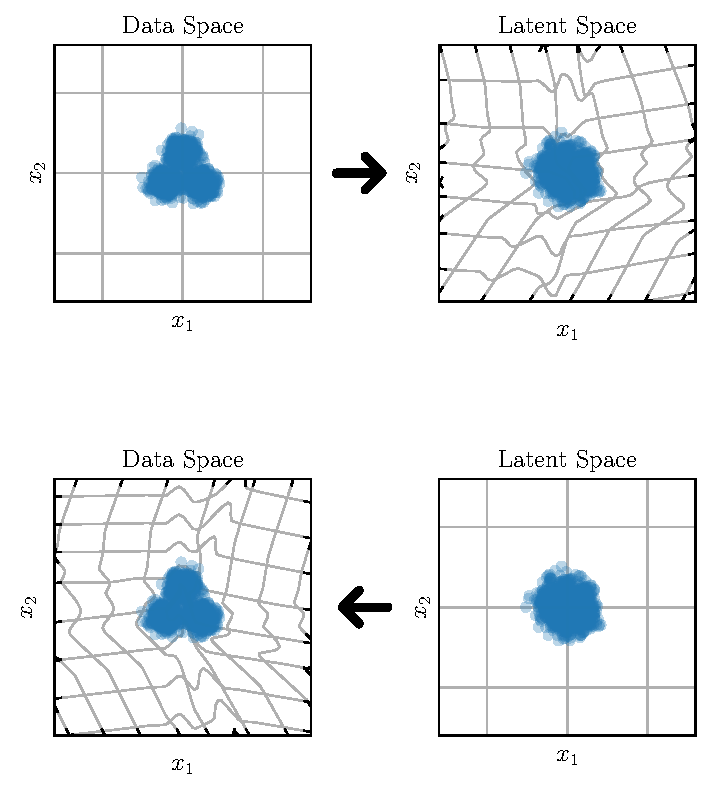
\includegraphics[height=0.7\textheight]{beamer-figures/toy_example/gaussian_mixture/grid_transformed.pdf}
        \caption{Mapping between data and latent space}%
    \end{figure}
\end{frame}

\begin{frame}{Theoretical Background}
    \framesubtitle{Extremal Sampling}
    
\begin{figure}[htpb]
	\centering
        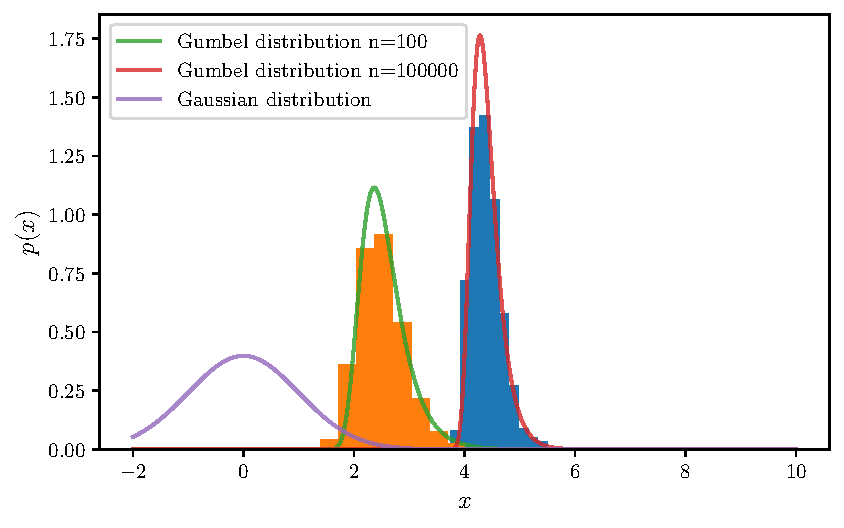
\includegraphics[height=0.7\textheight]{beamer-figures/samples/gumbel_uni.pdf}
	\caption{Gumbel distribution}%
	\label{fig:gumbel_uni}
\end{figure}
    
\end{frame}
\begin{frame}{Theoretical Background}
    \framesubtitle{Extremal Sampling}
    
\begin{equation}%
	\label{eq:sq_norm_chi}
	\lVert X \rVert_2 \sim \chi_d
\end{equation}

\begin{equation}
	\begin{aligned}%
		\label{eq:mean_var_sq_dist}
		\mathbb{E} \lVert X \rVert_2   & = \sqrt{2} \frac{\Gamma(\frac{d +
		1}{2})}{\Gamma(\frac{d}{2})}                                            \\
		\mathrm{Var} \lVert X \rVert_2 & = d - (\mathbb{E} \lVert X \rVert_2)^2
	\end{aligned}
\end{equation}
\end{frame}
\begin{frame}{Theoretical Background}
    \framesubtitle{Extremal Sampling}
    
\begin{figure}[htpb]
	\centering
        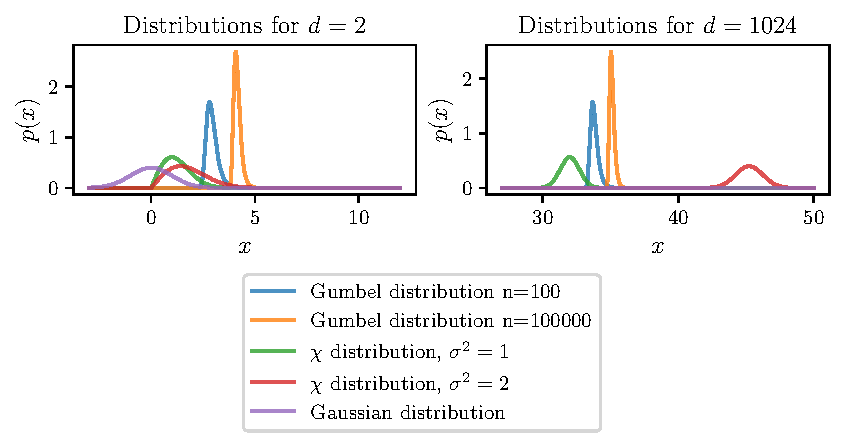
\includegraphics[height=0.7\textheight]{beamer-figures/samples/gumbel_multi.pdf}
	\caption{Gumbel distribution}%
        \label{fig:gumbel_multi}
\end{figure}
    
\end{frame}

\subsection{Archetypal Analysis}

\begin{frame}{Theoretical Background}
   \framesubtitle{Archetypal Analysis}
\begin{equation}%
    \label{eq:data_from_archetypes}
    \mathbf{x}_i = \sum_j a_{ij} \mathbf{z}_j
\end{equation}

\begin{equation}%
    \label{eq:archetypes_from_data}
    \mathbf{z}_j = \sum_i b_{ji} \mathbf{x}_i
\end{equation}

\begin{equation}
    \begin{aligned}%
        \label{eq:archetype_constraints}
        a_{ij} \geq 0 &\textrm{ and } \sum_{j=1}^{m} a_{ij} = 1 \\
        b_{ji} \geq 0 &\textrm{ and } \sum_{i=1}^{n} b_{ji} = 1
    \end{aligned}   
\end{equation}
\end{frame}
    
\begin{frame}{Theoretical Background}
   \framesubtitle{Archetypal Analysis}
\begin{equation}
    \begin{aligned}
        \label{eq:archetype_rss}
        \min_{a,b} \sum_i \lVert \mathbf{x}_i - \sum_j a_{ij} \mathbf{z}_j
        \rVert^2 \\
        = \min_{a,b} \sum_l \lVert \mathbf{x}_l - \sum_j a_{lj} \sum_i
        b_{ji} \mathbf{x}_i \rVert^2
    \end{aligned}
\end{equation}
\end{frame}

\begin{frame}{Theoretical Background}
    \framesubtitle{Archetypal Analysis}

    \begin{figure}[htpb]
        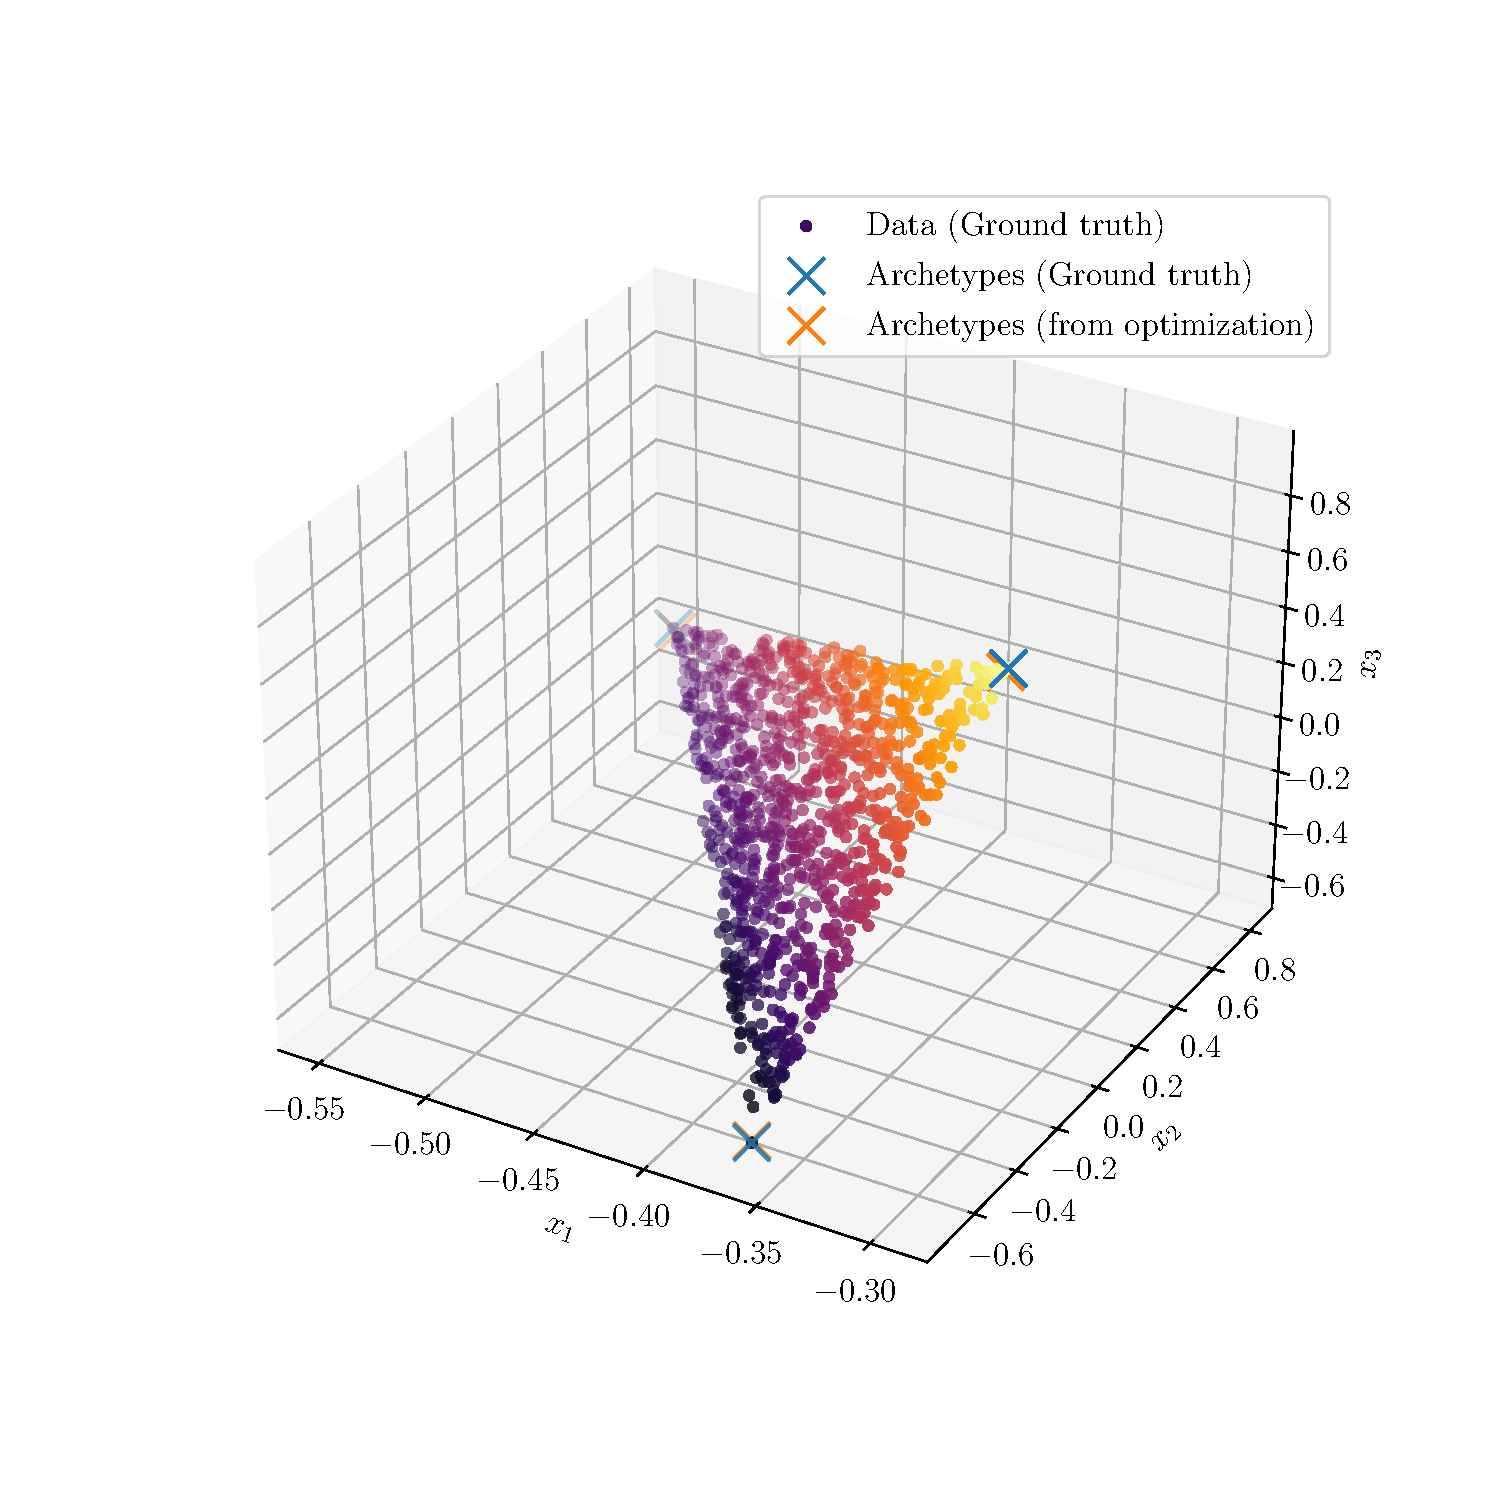
\includegraphics[height=0.7\textheight]{beamer-figures/aa_linear_toy.pdf}
        % \caption{Mapping between data and latent space}%
    \end{figure}
\end{frame}

\begin{frame}{Theoretical Background}
   \framesubtitle{DeepAA}
\begin{figure}[htpb]
	\begin{center}
		\begin{tikzpicture}[scale=1, transform shape]
			\node[varnode] (x) {$x$};
			\node[opnode] (inn) [right=of x] {INN};
			\node[varnode] (t) [right=of inn] {$t$};

			\node[opnode] (fa) at ($ (t) + (2cm,1cm) $) {$f_A$};
			\node[opnode] (fb) at ($ (t) + (2cm,-1cm) $) {$f_B$};

			\node[varnode] (A) [right=of fa] {$A$};
			\node[varnode] (B) [right=of fb] {$B$};

			\draw[grapharrow] (x)   -- (inn);
			\draw[grapharrow] (inn)   -- (t);
			\draw[grapharrow] (t)   -- (fa);
			\draw[grapharrow] (t)   -- (fb);
			\draw[grapharrow] (fa)   -- (A);
			\draw[grapharrow] (fb)   -- (B);
		\end{tikzpicture}
	\end{center}
	\caption{Forward pass of the normalizing flow with additional layers
		for the mapping to archetype coefficients.}%
	\label{fig:inn_aa_forward}
\end{figure}

\end{frame}

\begin{frame}{Theoretical Background}
   \framesubtitle{Sampling}
   \begin{figure}[htpb]
       \begin{center}
           \begin{tikzpicture}[scale=1, transform shape]
               \node[varnode] (x) {$x$};
               \node[opnode] (inn) [right=of x] {INN};
               \node[varnode] (t) [right=of inn] {$t$};

               \node[opnode] (fc) [right=of t] {$f_C$};

               \node[varnode] (ta) [right=of fc] {$t'$};

               \draw[grapharrow] (ta)   -- (fc);
               \draw[grapharrow] (fc)   -- (t);
               \draw[grapharrow] (t)   -- (inn);
               \draw[grapharrow] (inn)   -- (x);
           \end{tikzpicture}
       \end{center}
       \caption{Inverse computation from lower dimensional sample created from
       archetype coefficients to data space.}%
       \label{fig:inn_aa_backward}
   \end{figure}
   \begin{align*}
       A &\sim \mathrm{Dirichlet(c_1, \dots, c_k)}\\
       t' &= A z_{\mathrm{fixed}}
   \end{align*}
\end{frame}

\begin{frame}{Theoretical Background}
   \framesubtitle{Nullspace Sampling}
\begin{align*}
    A &= f_A(t) = \mathrm{softmax}(M_A t) \\
    t &= f_C(Az_{\mathrm{fixed}}) = M_C A z_{\mathrm{fixed}}
\end{align*}
\end{frame}

\begin{frame}{Theoretical Background}
   \framesubtitle{Nullspace Sampling}
\begin{align*}
    A &= M_A t \\
    t &= M_A^+ A + [I - M_A^+ M_A] \mathbf{w}
\end{align*}
\end{frame}

\begin{frame}{Theoretical Background}
   \framesubtitle{Nullspace Sampling}
\begin{align*}
    t &= f_C(Az_{\mathrm{fixed}}) + [I - M_A^+ M_A] \mathbf{w}
\end{align*}
\end{frame}

\subsection{Discriminator and Classifier Training}
\begin{frame}{Theoretical Background}
   \framesubtitle{Discriminator Training}
\begin{equation}
	\mathbb{E}_{\hat{x}, \hat{y} \sim p_{\mathrm{in}}} \log D(x, y) +
	\mathbb{E}_{z \sim p_{\mathrm{out}}} \log ( 1 - D(z, y) )
\end{equation}
\end{frame}
\begin{frame}{Theoretical Background}
   \framesubtitle{Classifier Training}
\begin{equation}
	\mathbb{E}_{\hat{x}, \hat{y} \sim p_{\mathrm{in}}} \log p(y=\hat{y} | \hat{x}) -
	\beta \mathbb{E}_{z \sim p_{\mathrm{out}}} \mathrm{KL}(\mathcal{U}(y) | p(y | z))
\end{equation}
\end{frame}


\section{Experiments}

\subsection{Toy Data}

\begin{frame}{Toy Data}
    \begin{figure}
        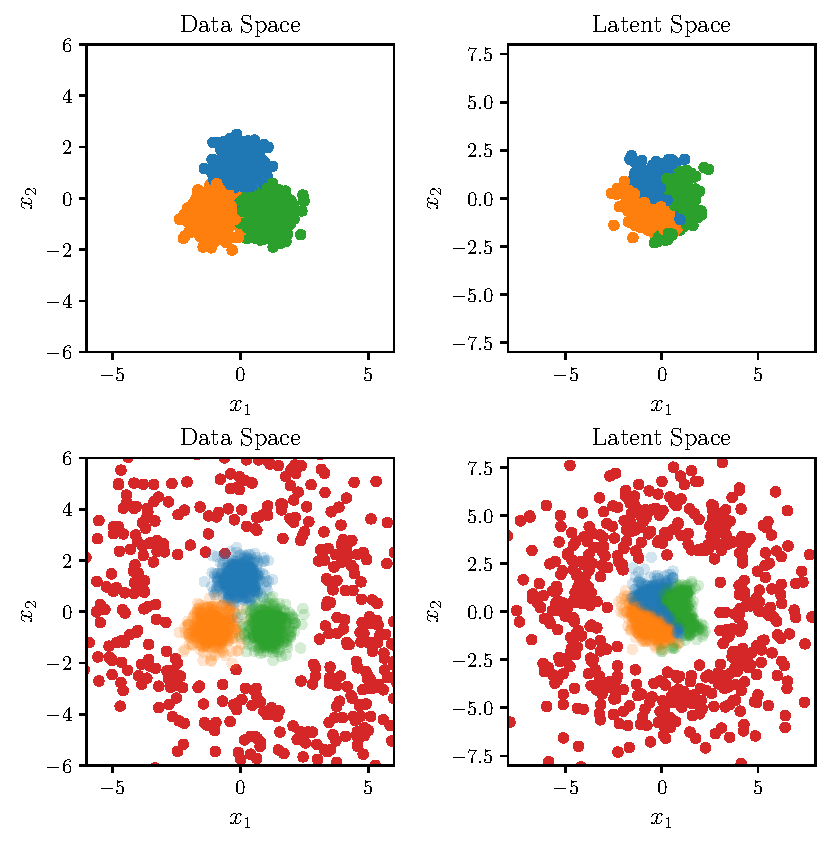
\includegraphics[height=0.7\textheight]{beamer-figures/toy_example/gaussian_mixture/latent_mapping.pdf}
    \end{figure}
\end{frame}
\begin{frame}{Toy Data}
    \begin{figure}
        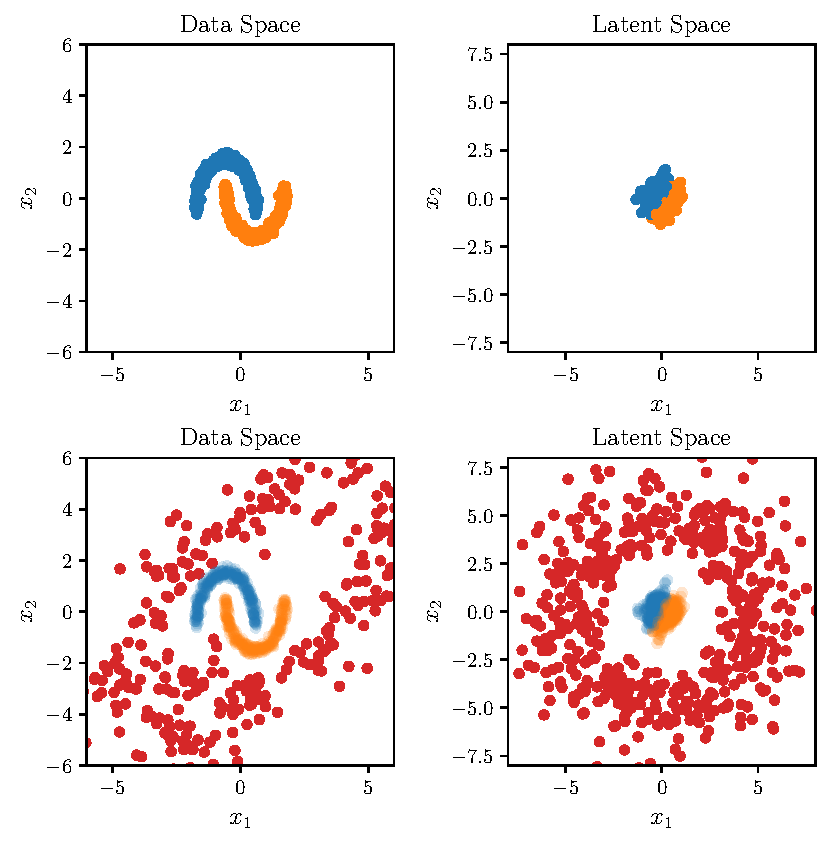
\includegraphics[height=0.7\textheight]{beamer-figures/toy_example/moons/latent_mapping.pdf}
    \end{figure}
\end{frame}

\begin{frame}{Toy Data}
    \framesubtitle{Classifier}
    \begin{figure}
        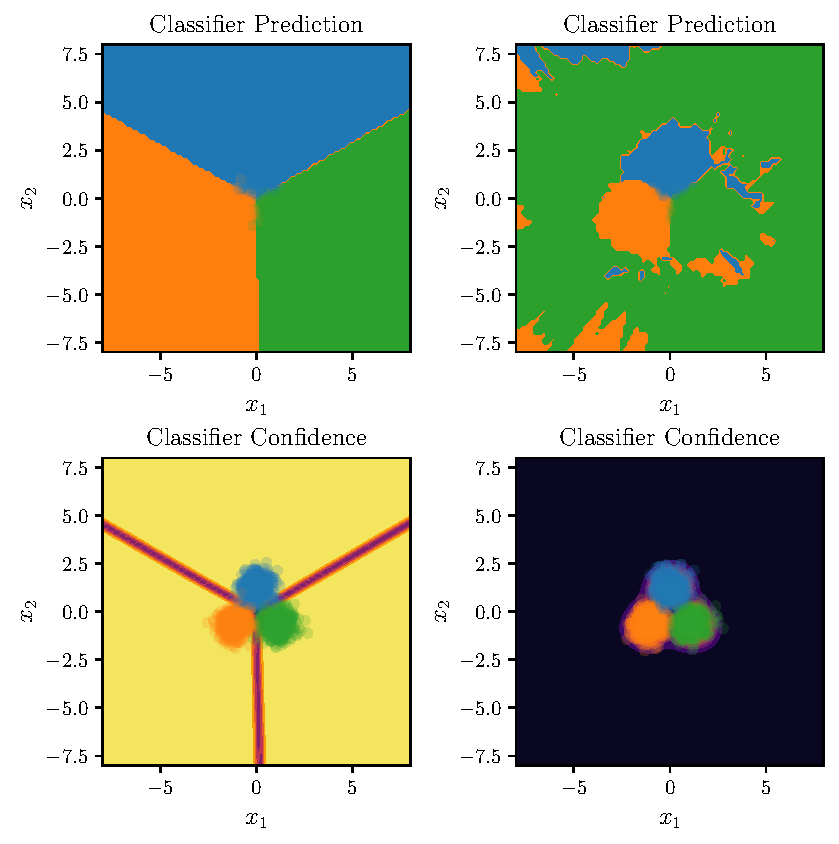
\includegraphics[height=0.7\textheight]{beamer-figures/toy_example/gaussian_mixture/classifier.pdf}
    \end{figure}
\end{frame}
\begin{frame}{Toy Data}
    \framesubtitle{Classifier}
    \begin{figure}
        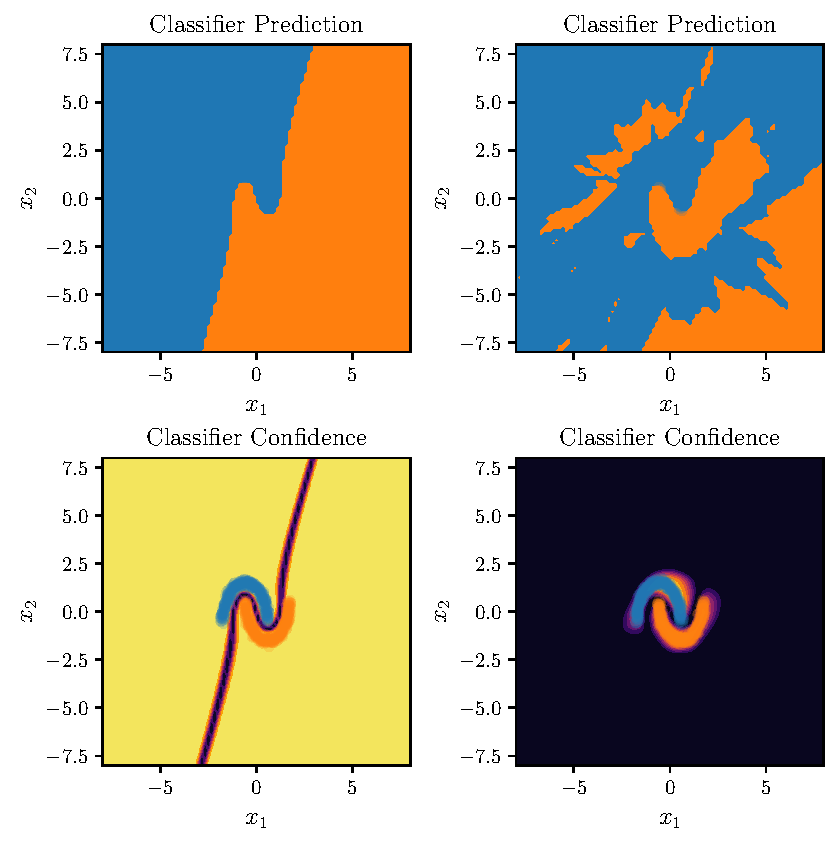
\includegraphics[height=0.7\textheight]{beamer-figures/toy_example/moons/classifier.pdf}
    \end{figure}
\end{frame}

\subsection{Qualitative Comparison}

\begin{frame}{EMNIST}
    \begin{figure}
        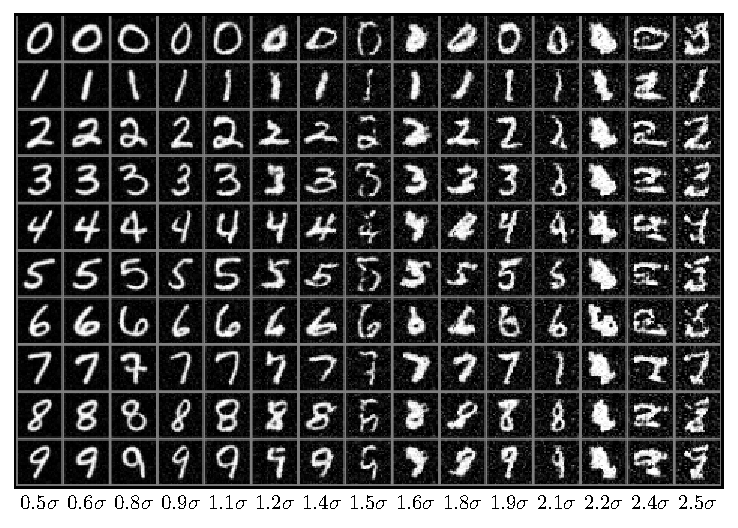
\includegraphics[height=0.7\textheight]{beamer-figures/samples/samples_increasing_distance_EMNIST.pdf}
    \end{figure}
\end{frame}
\begin{frame}{FERG}
    \begin{figure}
        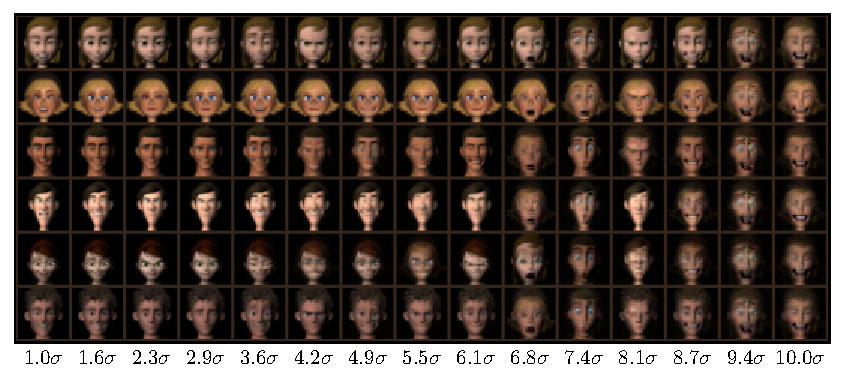
\includegraphics[height=0.7\textheight]{beamer-figures/samples/samples_increasing_distance_FERG_people.pdf}
    \end{figure}
\end{frame}

\subsection{Archetypal Analysis}

\begin{frame}{Number of Archetypes for Digits}
\begin{figure}[htpb]
	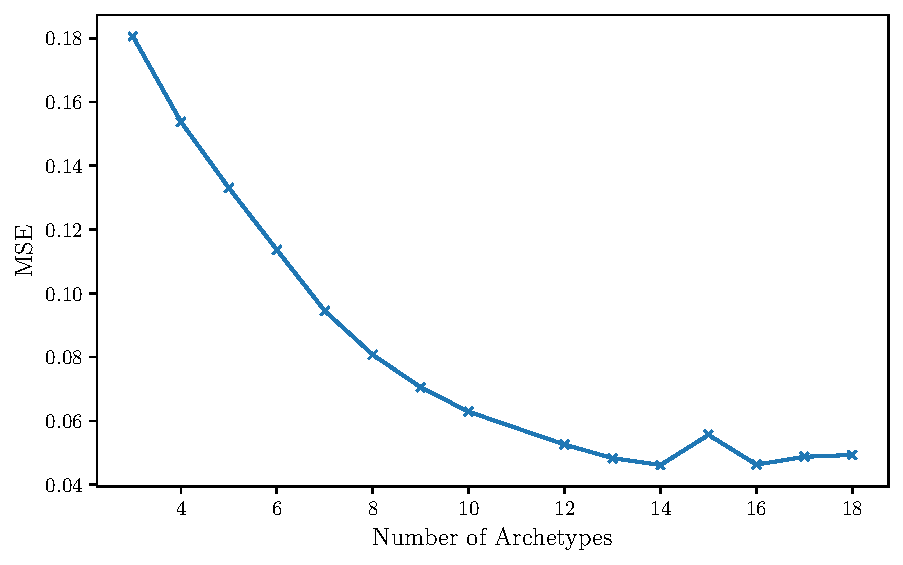
\includegraphics[height=0.7\textheight]{figures/samples/aa_mse_EMNIST.pdf}
\end{figure}
\end{frame}

\begin{frame}{Number of Archetypes for People}
\begin{figure}[htpb]
	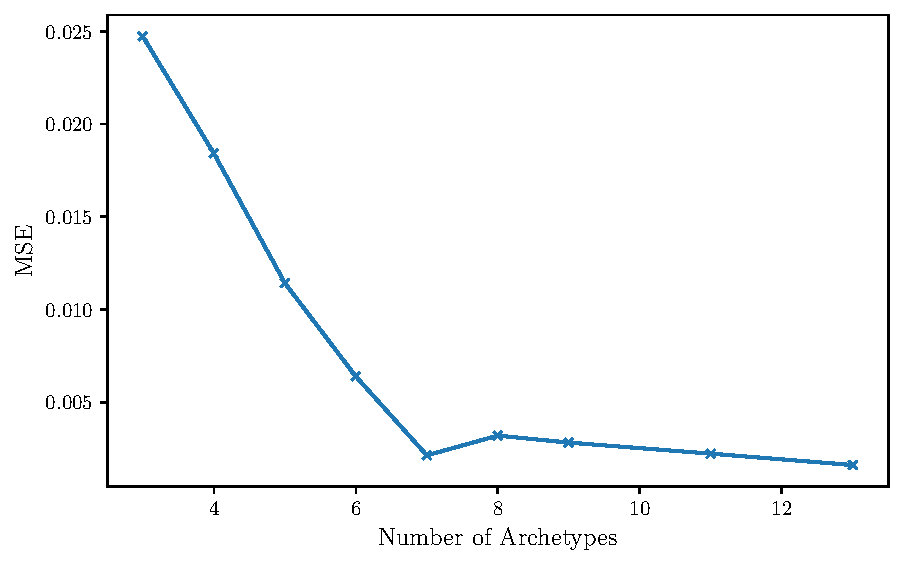
\includegraphics[height=0.7\textheight]{figures/samples/aa_mse_FERG.pdf}
\end{figure}
\end{frame}

\begin{frame}{Archetypes (Digits)}
\begin{figure}[htpb]
	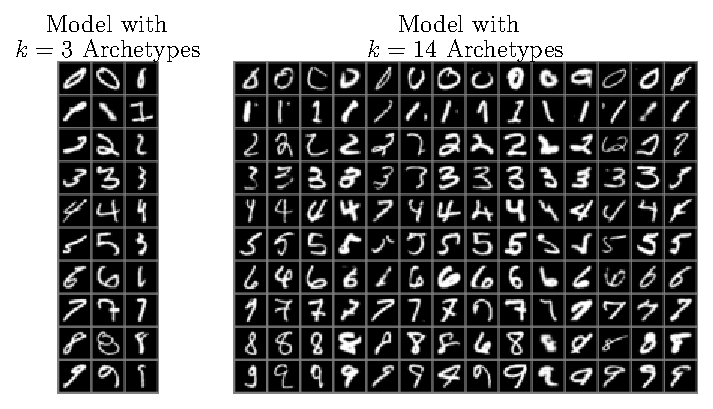
\includegraphics[height=0.7\textheight]{beamer-figures/samples/archetypes_emnist.pdf}
\end{figure}
\end{frame}

\begin{frame}{Archetypes (People)}
\begin{figure}[htpb]
	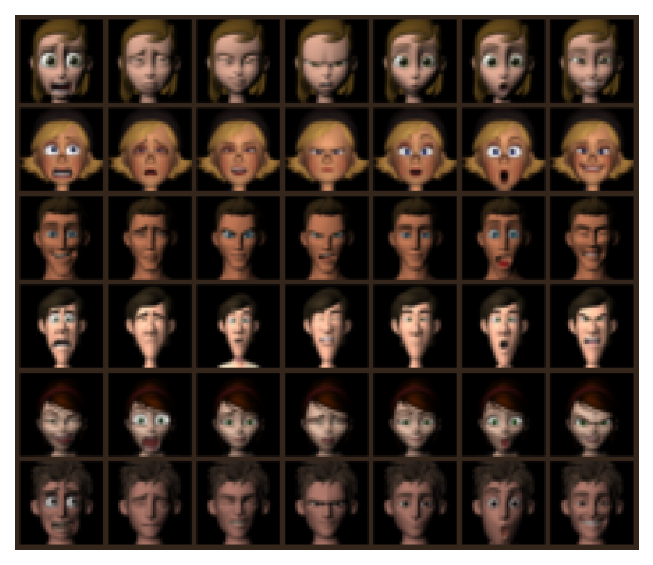
\includegraphics[height=0.7\textheight]{figures/samples/archetypes_ferg_7.pdf}
\end{figure}
\end{frame}

\begin{frame}{Sampling Inliers (Digits)}
\begin{figure}[htpb]
	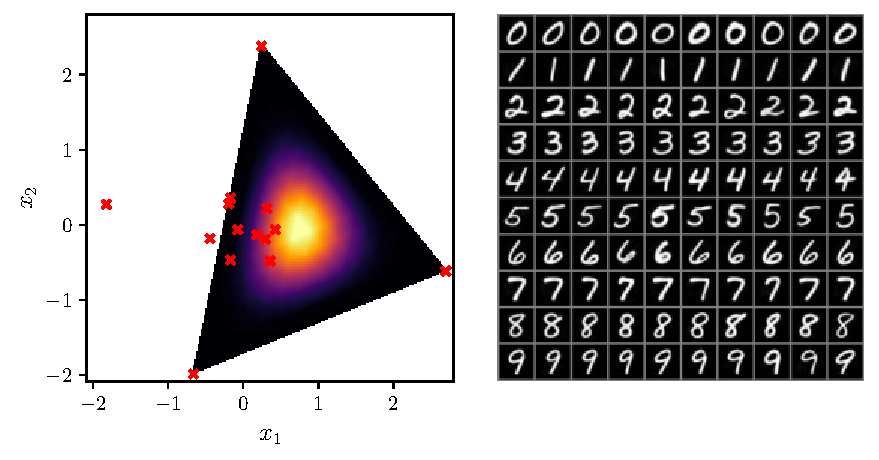
\includegraphics[height=0.7\textheight]{figures/samples/aa_emnist.pdf}
\end{figure}
\end{frame}

\begin{frame}{Sampling Outliers (Digits)}
\begin{figure}[htpb]
	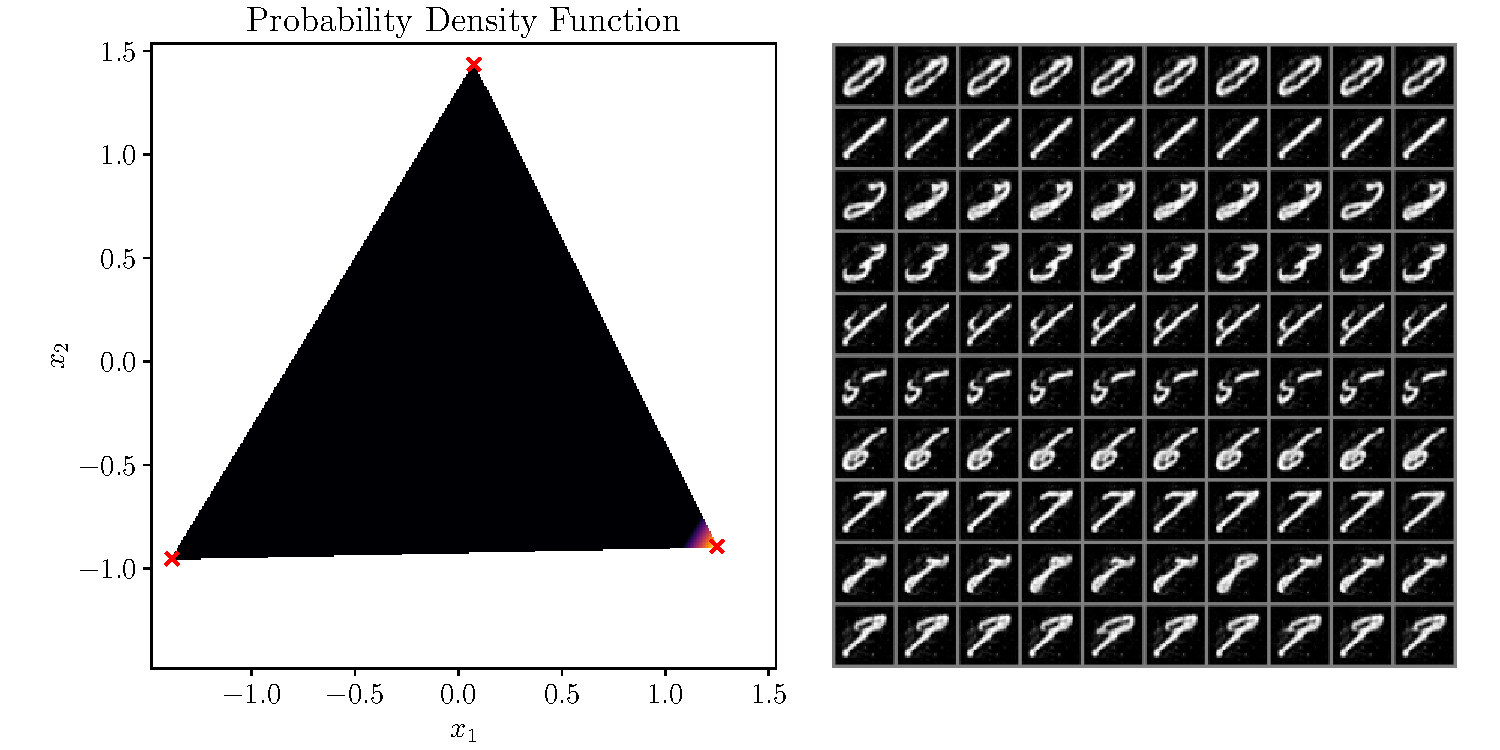
\includegraphics[height=0.7\textheight]{figures/samples/aa_emnist1.pdf}
\end{figure}
\end{frame}

\begin{frame}{Sampling Outliers (Digits)}
\begin{figure}[htpb]
	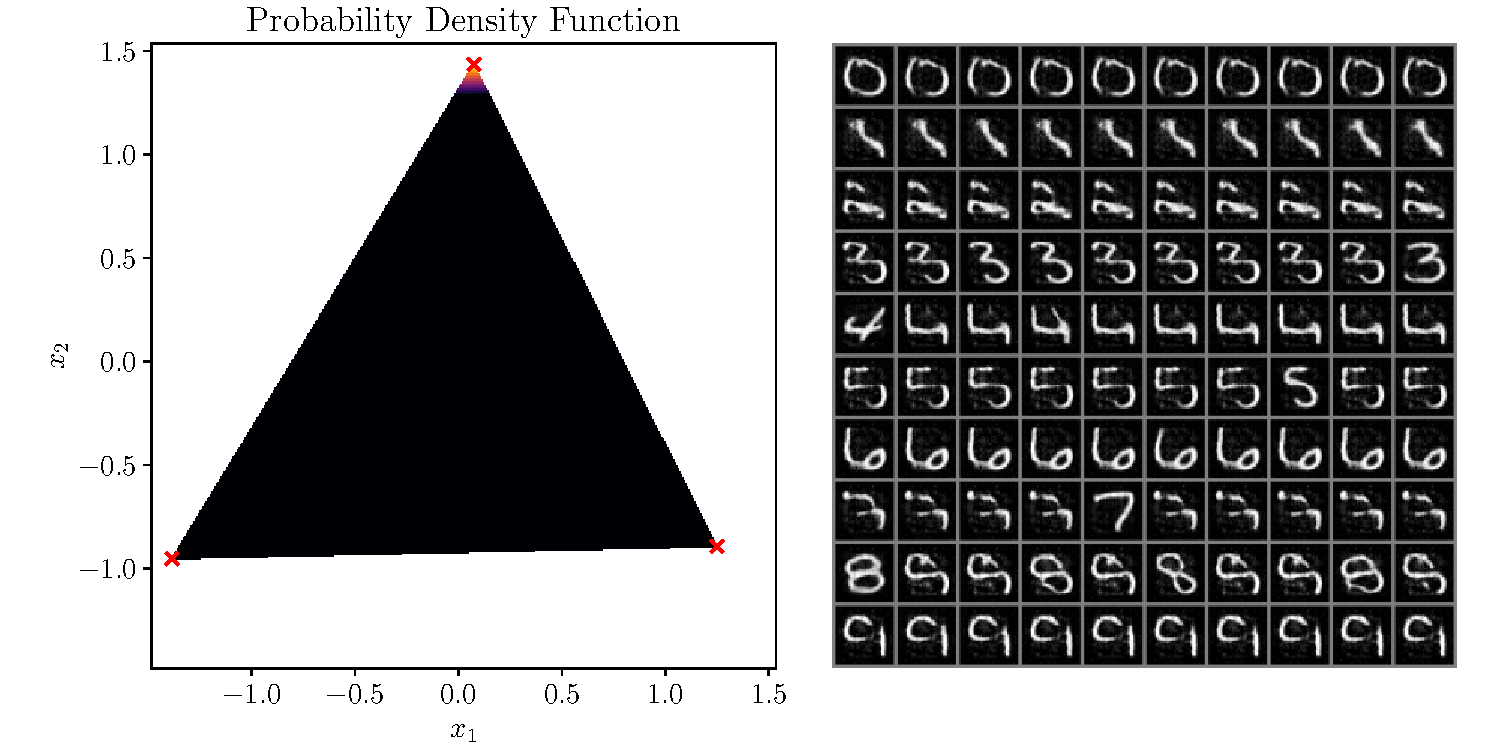
\includegraphics[height=0.7\textheight]{figures/samples/aa_emnist2.pdf}
\end{figure}
\end{frame}

\begin{frame}{Sampling Outliers (Digits)}
\begin{figure}[htpb]
	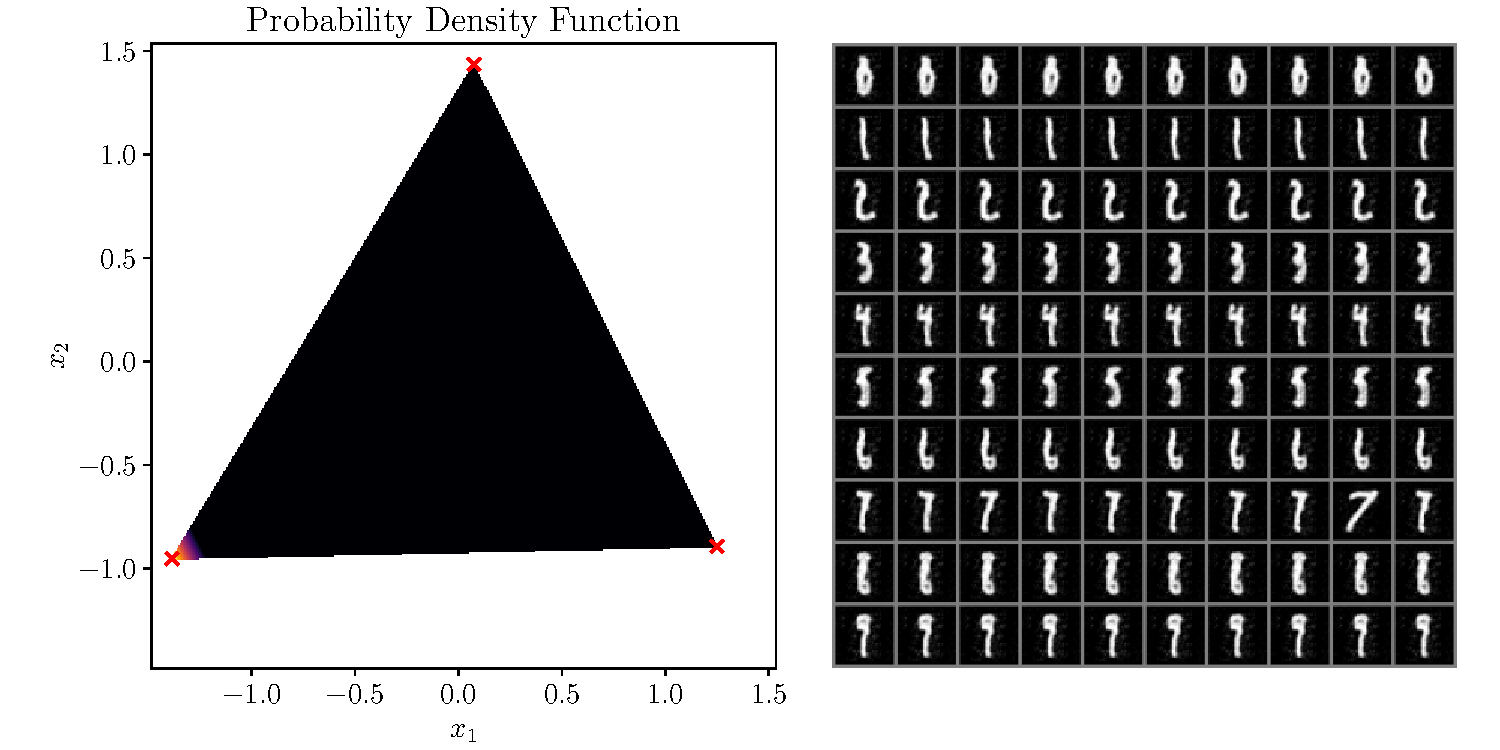
\includegraphics[height=0.7\textheight]{figures/samples/aa_emnist3.pdf}
\end{figure}
\end{frame}

\begin{frame}{Sampling Inliers (People)}
\begin{figure}[htpb]
	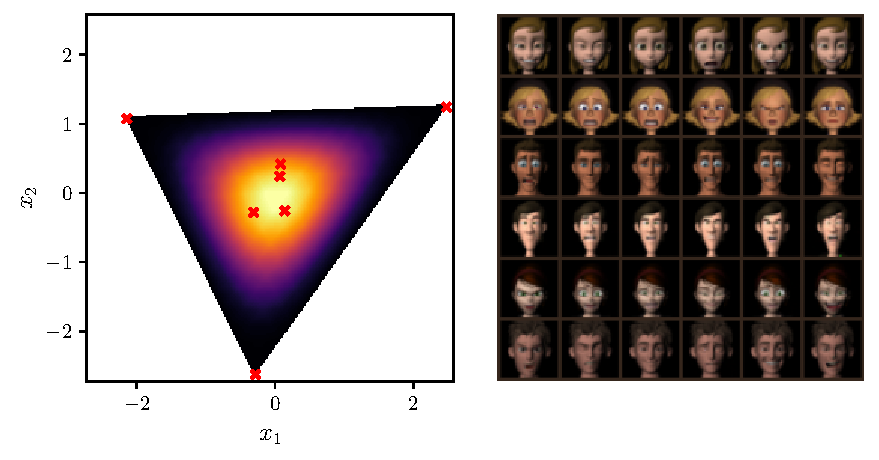
\includegraphics[height=0.7\textheight]{figures/samples/aa_ferg.pdf}
\end{figure}
\end{frame}

\begin{frame}{Sampling Outliers (People)}
\begin{figure}[htpb]
	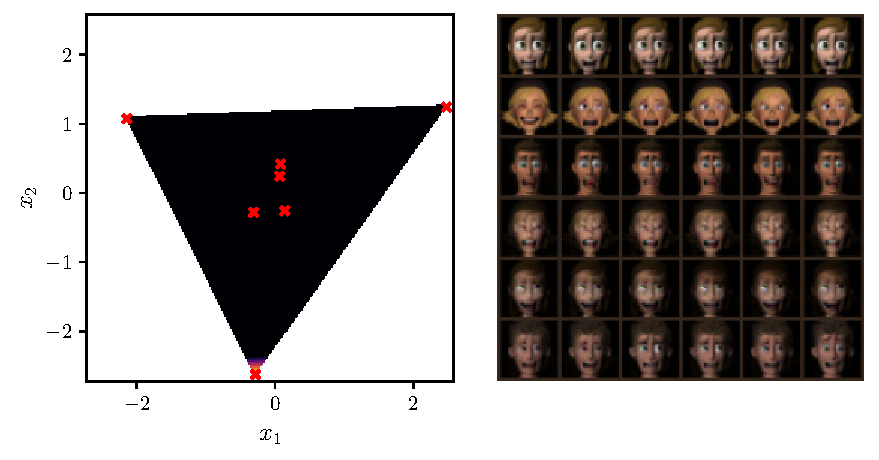
\includegraphics[height=0.7\textheight]{figures/samples/aa_ferg1.pdf}
\end{figure}
\end{frame}

\begin{frame}{Sampling Outliers (People)}
\begin{figure}[htpb]
	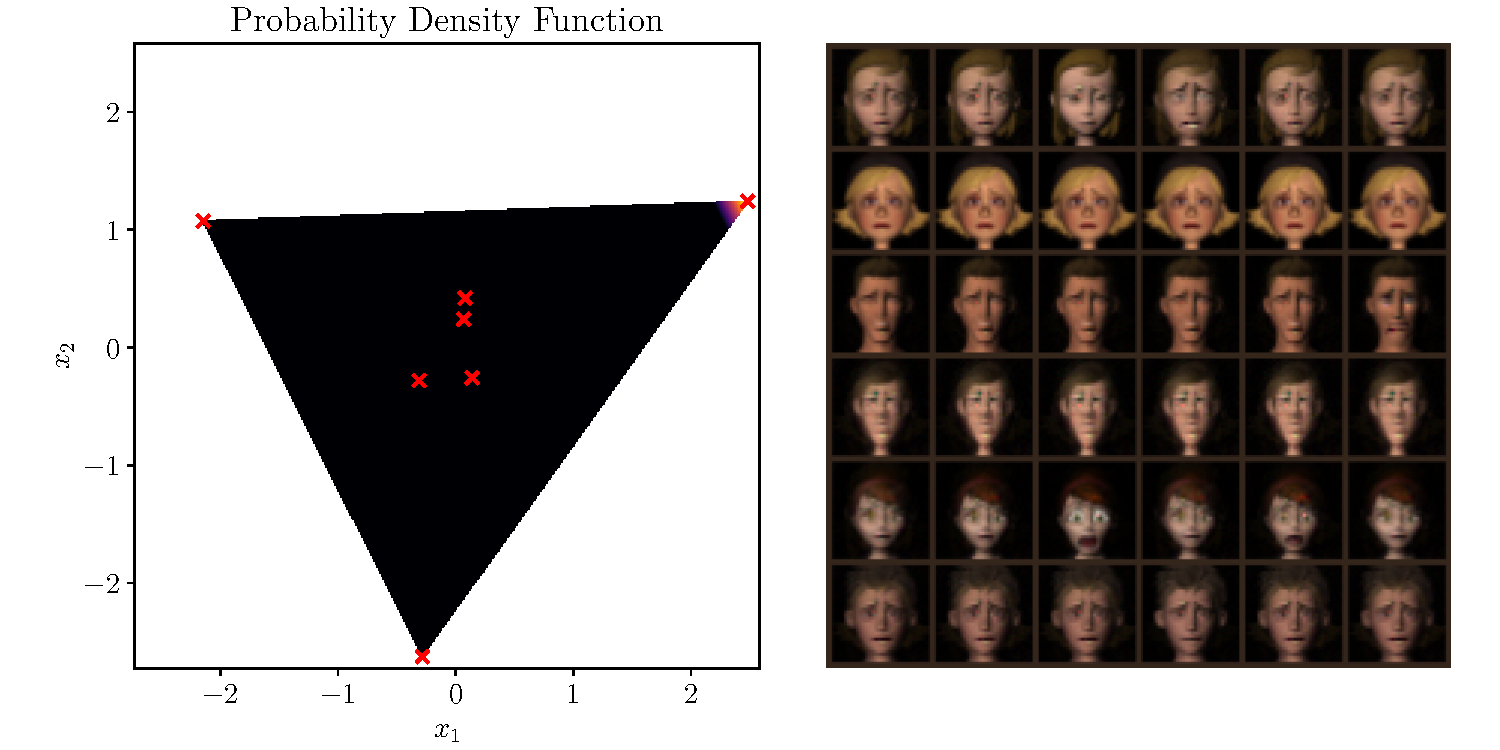
\includegraphics[height=0.7\textheight]{figures/samples/aa_ferg2.pdf}
\end{figure}
\end{frame}

\begin{frame}{Sampling Outliers (People)}
\begin{figure}[htpb]
	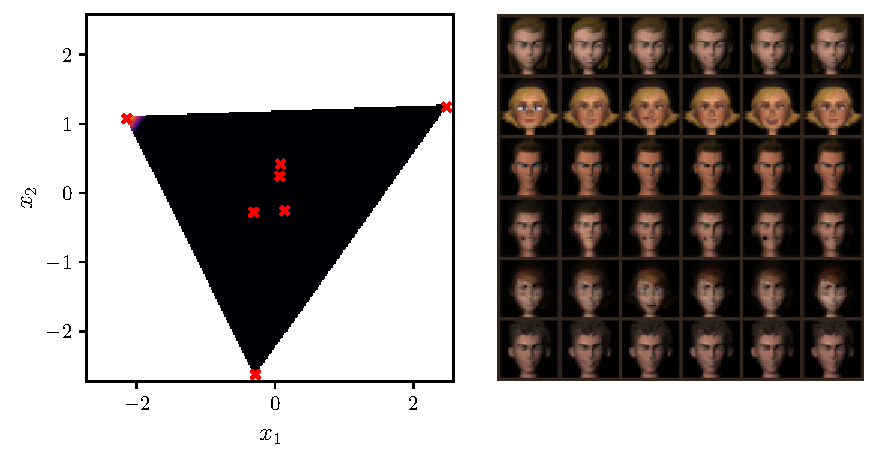
\includegraphics[height=0.7\textheight]{figures/samples/aa_ferg3.pdf}
\end{figure}
\end{frame}

\begin{frame}{Sampling with Nullspace}
\begin{figure}[htpb]
	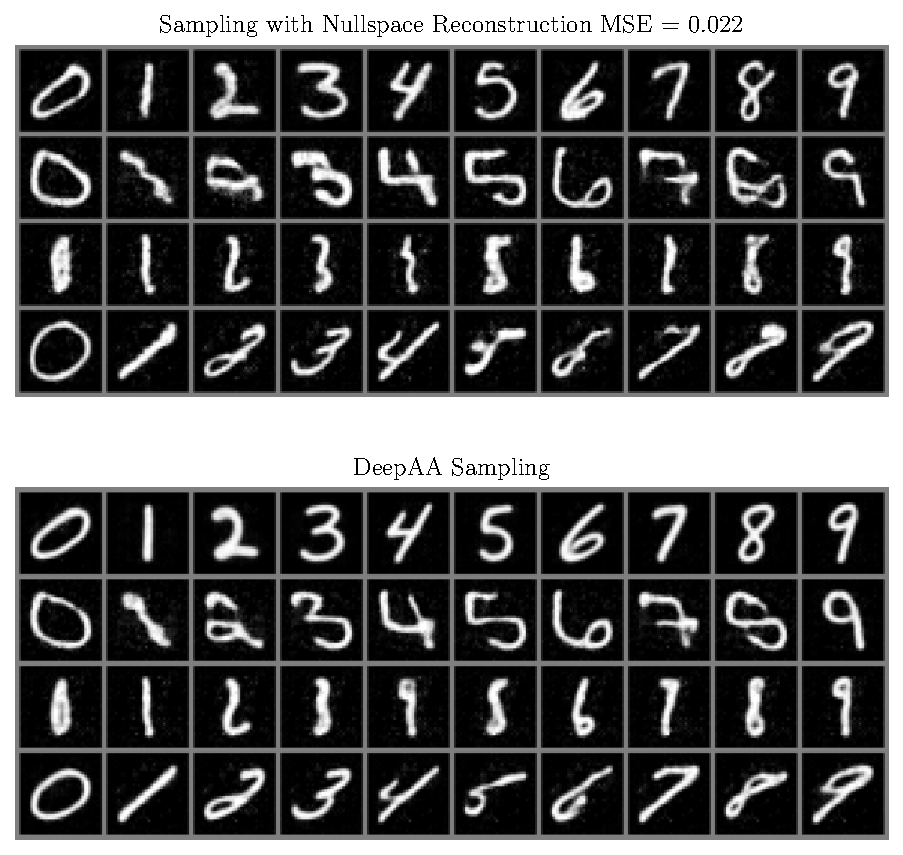
\includegraphics[height=0.7\textheight]{figures/samples/aa_nullspace.pdf}
\end{figure}
\end{frame}

\begin{frame}{Sampling with Nullspace (biased)}
\begin{figure}[htpb]
	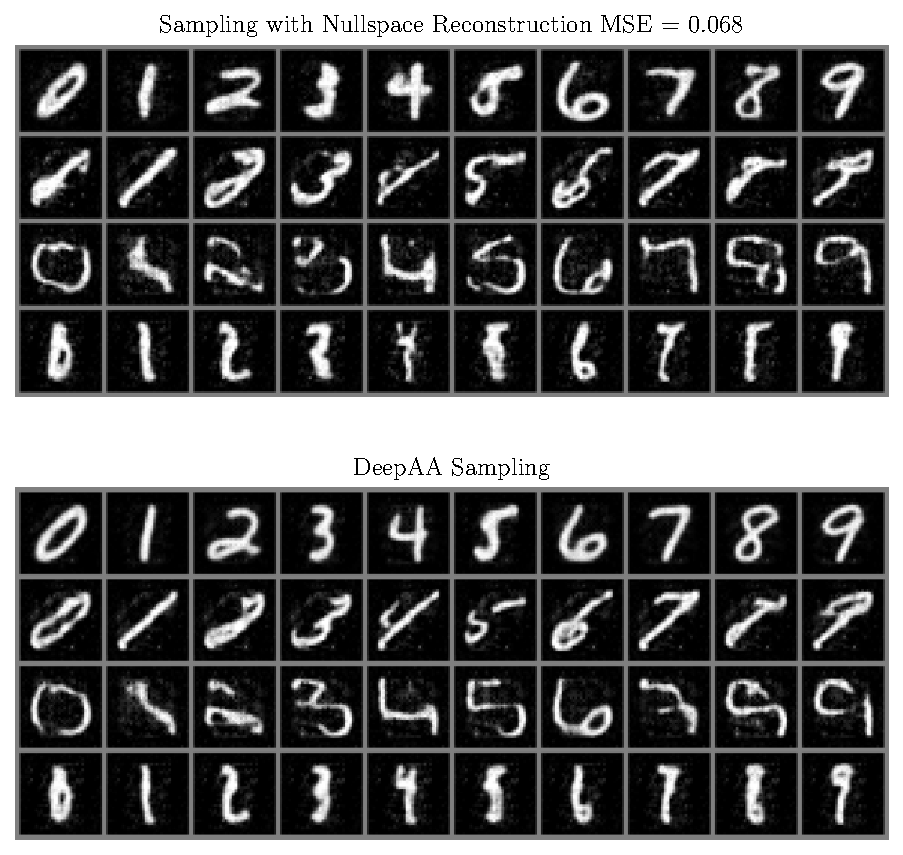
\includegraphics[height=0.7\textheight]{figures/samples/aa_nullspace_bias_y.pdf}
\end{figure}
\end{frame}

\subsection{Analysis of the Latent Space}

\begin{frame}{Cluster Distance between Classes}
\begin{figure}[htpb]
	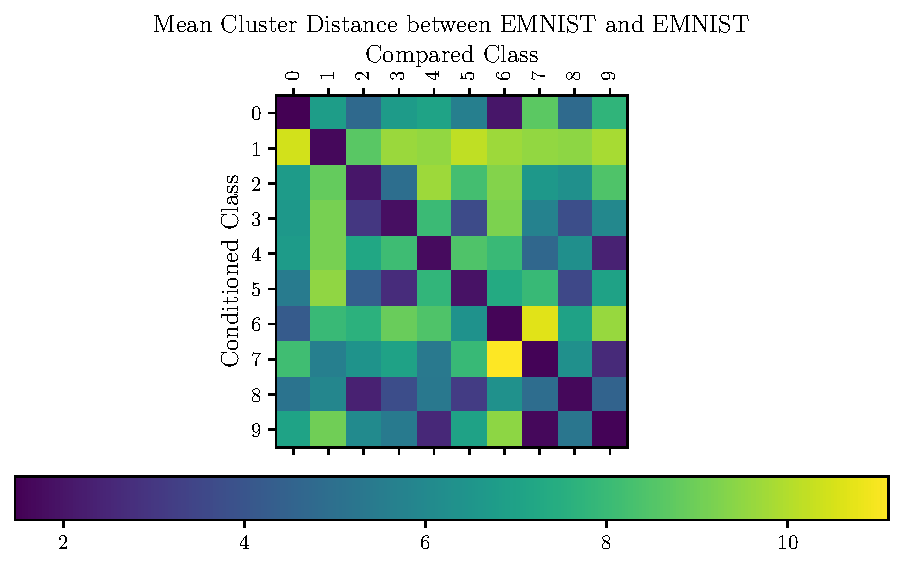
\includegraphics[height=0.7\textheight]{figures/samples/emnist_distance_matrix_EMNIST_lda.pdf}
\end{figure}
\end{frame}

\begin{frame}{Cluster Distance between Classes}
\begin{figure}[htpb]
	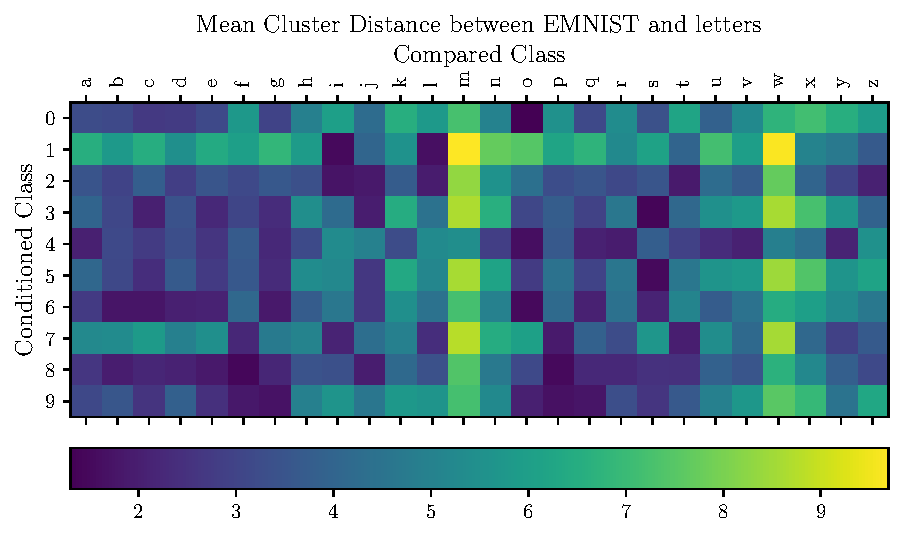
\includegraphics[height=0.7\textheight]{figures/samples/emnist_distance_matrix_letters_lda.pdf}
\end{figure}
\end{frame}

\begin{frame}{Distribution of Latent Space Radii}
\begin{figure}[htpb]
	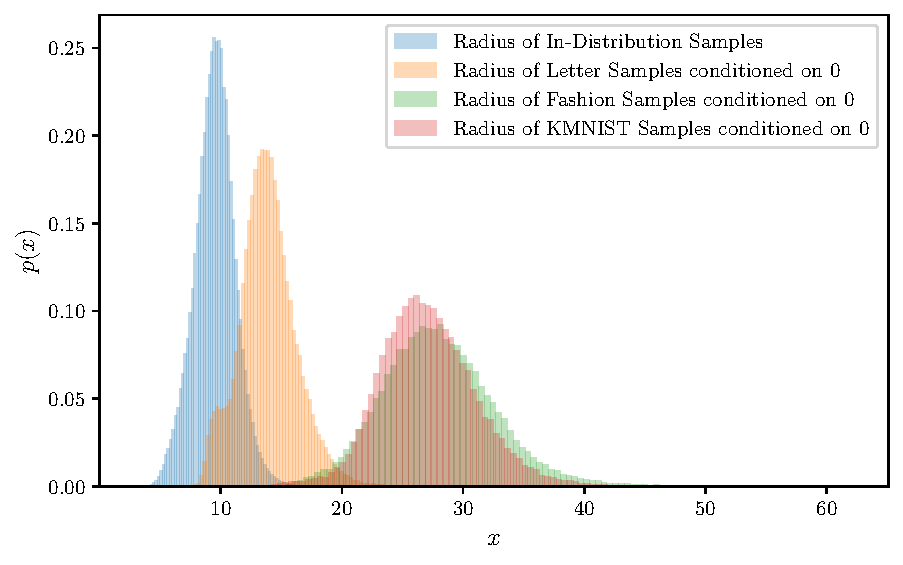
\includegraphics[height=0.7\textheight]{figures/samples/emnist_radius_hist.pdf}
\end{figure}
\end{frame}

\begin{frame}{Distribution of Latent Space Radii}
\begin{figure}[htpb]
	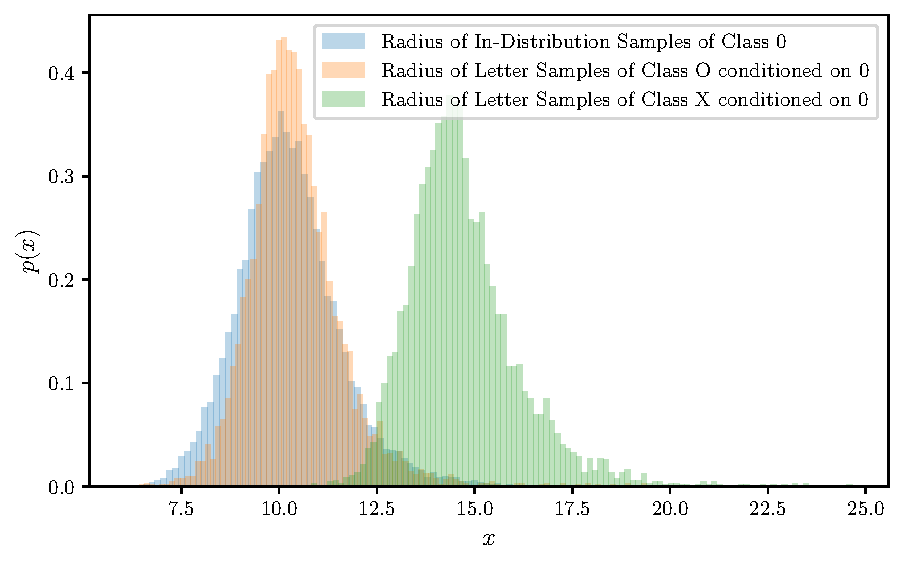
\includegraphics[height=0.7\textheight]{figures/samples/emnist_radius_hist_xo.pdf}
\end{figure}
\end{frame}

\subsection{Discriminator Performance}

\begin{frame}{Discriminator Performance}
\begin{table}[htpb]
\begin{tabular}{lrrrrrr}
\toprule
{outliers} & \multicolumn{2}{c}{letters} & \multicolumn{2}{c}{fashion} & \multicolumn{2}{c}{kmnist} \\
{metric} & {AUC} & {AP} & {AUC} & {AP} & {AUC} & {AP} \\
\midrule
DeepAA, p = 0.1 & 0.64 & 0.33 & 0.88 & 0.77 & 0.67 & 0.47 \\
DeepAA, p = 0.3 & 0.57 & 0.27 & 0.52 & 0.37 & 0.46 & 0.34 \\
DeepAA, p = 0.5 & 0.48 & 0.22 & 0.38 & 0.31 & 0.42 & 0.33 \\
DeepAA, p = 0.6 & 0.47 & 0.22 & 0.39 & 0.32 & 0.37 & 0.31 \\
DeepAA, p = 0.8 & 0.43 & 0.20 & 0.48 & 0.35 & 0.39 & 0.32 \\
DeepAA, p = 1.2 & 0.45 & 0.21 & 0.74 & 0.51 & 0.63 & 0.42 \\
INN, Gumbel, p = 2.5 & 0.68 & 0.35 & 0.45 & 0.34 & 0.47 & 0.35 \\
INN, Normal, p = 1.5 & 0.58 & 0.27 & 0.12 & 0.25 & 0.38 & 0.32 \\
INN, Normal, p = 2.0 & 0.65 & 0.32 & 0.20 & 0.27 & 0.48 & 0.35 \\
INN, Normal, p = 2.5 & 0.69 & 0.39 & 0.80 & 0.61 & 0.72 & 0.50 \\
INN, Normal, p = 3.0 & 0.52 & 0.24 & 0.42 & 0.33 & 0.15 & 0.25 \\
fashion & 0.73 & 0.44 & \bfseries 1.00 & \bfseries 1.00 & \bfseries 0.97 & \bfseries 0.95 \\
letters & \bfseries 0.81 & \bfseries 0.56 & 0.50 & 0.36 & 0.48 & 0.35 \\
\bottomrule
\end{tabular}
\end{table}
\end{frame}

\begin{frame}{Classifier Performance}
\begin{table}[htpb]
	\begin{tabular}{lrrrrrrrrr}
\toprule
{outliers} & \multicolumn{3}{c}{letters} & \multicolumn{3}{c}{fashion} & \multicolumn{3}{c}{kmnist} \\
{metric} & {AUC} & {AP} & {ACC} & {AUC} & {AP} & {ACC} & {AUC} & {AP} & {ACC} \\
\midrule
DeepAA, p = 0.1 & 0.89 & 0.64 & 1.00 & 1.00 & 1.00 & 1.00 & 0.99 & 0.98 & 1.00 \\
DeepAA, p = 0.3 & 0.90 & 0.66 & \bfseries 1.00 & 1.00 & 1.00 & \bfseries 1.00 & 0.99 & 0.99 & \bfseries 1.00 \\
DeepAA, p = 0.6 & 0.89 & 0.63 & 1.00 & 1.00 & 1.00 & 1.00 & 0.98 & 0.97 & 1.00 \\
DeepAA, p = 0.8 & 0.90 & 0.68 & 1.00 & 1.00 & 1.00 & 1.00 & 0.98 & 0.98 & 1.00 \\
DeepAA, p = 1.0 & 0.89 & 0.70 & 0.99 & 1.00 & 1.00 & 0.99 & 0.97 & 0.96 & 0.99 \\
DeepAA, p = 1.2 & 0.89 & 0.68 & 1.00 & 1.00 & 1.00 & 1.00 & 0.98 & 0.96 & 1.00 \\
INN, Gumbel, p = 2.5 & 0.90 & 0.72 & 1.00 & 1.00 & 1.00 & 1.00 & \bfseries 0.99 & \bfseries 0.99 & 1.00 \\
fashion & 0.89 & 0.67 & 1.00 & \bfseries 1.00 & \bfseries 1.00 & 1.00 & 0.99 & 0.99 & 1.00 \\
letters & \bfseries 0.98 & \bfseries 0.95 & 1.00 & 1.00 & 1.00 & 1.00 & 0.99 & 0.99 & 1.00 \\
none & 0.89 & 0.68 & 0.99 & 1.00 & 1.00 & 0.99 & 0.97 & 0.95 & 0.99 \\
\bottomrule
\end{tabular}

\end{table}
\end{frame}

\subsection{Conclusion}

\begin{frame}{Conclusion}
    \begin{itemize}
        \item INNs/Normalizing Flows well suited for outlier generation
        \item Archetypal Analysis interesting approach for interpretable latent
            space
    \end{itemize}
\end{frame}

\subsection{Future Work}

\begin{frame}{Future Work}
    \begin{itemize}
        \item Use bigger models to test on ImageNet
        \item Work unconditionally
        \item Goal: Completely unsupervised model of outliers
    \end{itemize}
\end{frame}

\end{document}
